\documentclass{article}
\usepackage[utf8]{inputenc}
\usepackage[vietnamese, main=english]{babel}
\usepackage{graphicx}
\usepackage{hyperref}
\usepackage{minted}

\hypersetup{
	colorlinks=true,
	urlcolor=blue
}

\begin{document}
\begin{titlepage}
	\title{
		\Large{Distributed System - Practical work 1} \\
		\Huge{\textbf{TCP File transfer}} \\
		\includegraphics[width=0.4\textwidth]{logo-usth-pa3-01.png}
	}
	\author{
		\selectlanguage{vietnamese} Ngô Ngọc Đức Huy -- BI9-119 \\
	}
	\date{\today}
\end{titlepage}

\maketitle

\section{Protocol}

We modify the provided simple chat system to make this file transfering system.
In this proof-of-concept we only concerns the file sending from the client to the server.

After the initial request for connection being accepted, the client sends to the server
the file's metadata:

\begin{itemize}
	\item file size, so that the server knows how many packets to receive
	\item file name, so that the server knows what to save as
\end{itemize}

The client consequently sends chunks of data until all the file is sent.
After that, it prompts to disconnect with the server.

\begin{figure}
	\centering
	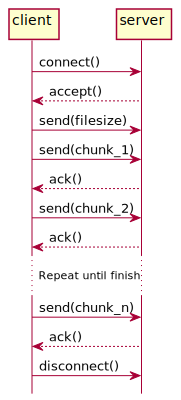
\includegraphics{pw1/protocol.pdf}
	\caption{Our protocol for file transfering}
\end{figure}

\section{System organization}

In this system, the client and the server each has a program dedicated for sending or receiving
and a file system. The sender program reads the file at the client and send it to the server
using TCP/IP protocol. The receiver program at the server writes to a file upon receiving the data.

\begin{figure}
	\centering
	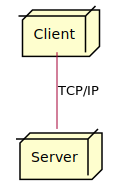
\includegraphics{pw1/system-org.pdf}
	\caption{The system organization}
\end{figure}

\section{Implementation}

According to the above design, \selectlanguage{vietnamese} Nguyễn Gia Phong \selectlanguage{english} has implemented this system.
In this section we will clarify how this implementation reflects the design.

\subsection{Client}

The program first reads the file name from command line input.
The filesize is stored as a string rather than integer
because different systems can have different ways to handle numbers' endianness,
which may lead to error. The file size is limited to 1GiB.

Afterwards, the file size and the file name are sent.

\begin{minted}{c}
	const char *fname = argv[1];
	char fsize[10];
	struct stat st;
	stat(fname, &st);

	sprintf(fsize, "%ld", st.st_size);
	send(sockfd, fsize, 10, 0);

	char name_trunc[16];
	strncpy(name_trunc, fname, 15);
	name_trunc[15] = 0;
	send(sockfd, name_trunc, 16, 0);
\end{minted}

After that, the client iteratively reads data chunks from the file and send it:

\begin{minted}{c}
	FILE *f = fopen(fname, "r");
	char chunk[CHUNK_SIZE];
	int len;
	while (len = fread(chunk, 1, CHUNK_SIZE, f)) {
		send(sockfd, chunk, len, 0);
		/* Avoid filling kernel buffer */
		recv(sockfd, chunk, 1, 0);
	}
\end{minted}

\subsection{Server}

On the server size, after initiating the socket and getting ready for listening,
the server runs an infinite while loop. Inside it, the server waits until a client
requests to connect, upon which it forks so that it can continue
to wait for another client.

\begin{minted}{c}
	int cli = accept(ss, (struct sockaddr *)&ad, &ad_length);
	if (fork())
		continue;
\end{minted}

Since \texttt{fork()} returns 0 on the child process and the child's process ID
on the parent process, the parent process will \texttt{continue} and wait for a client,
while the child process the incoming data. Firstly, it receives the file size and file name:

\begin{minted}{c}
	char fsize[10];
	recv(cli, fsize, 10, 0);
	int size;
	sscanf(fsize, "%d", &size);

	char fname[16];
	recv(cli, fname, 16, 0);
	puts(fname);
	FILE *f = fopen(fname, "w");
\end{minted}

After receiving the metadata, it will continue to receive the chunks sent from client:

\begin{minted}{c}
	int len;
	while (len = recv(cli, chunk, CHUNK_SIZE, 0)) {
		fwrite(chunk, 1, len, f);
		send(cli, ACK, 1, 0);
	}
\end{minted}

Finally, the child process closes the connection and terminates:

\begin{minted}{c}
	fclose(f);
	close(cli);
	return 0;
\end{minted}

\subsection{Source code}

The full implementation can be found as \texttt{client.c} and \texttt{server.c} on
our \href{https://github.com/Huy-Ngo/ds2021/tree/master/pw1}{GitHub repository}.

\end{document}
